%!TEX root = master.tex

\section{Anhang}

%%%
%%% Anhang
%%%

\begin{frame}
  \frametitle{Anhang}
\end{frame}

%%%
%%% Szenario Log
%%%

\begin{frame}
  \frametitle{Anhang - Szenario Logarithmic}
  Dieses Szenario implementiert zum Vergleich ein logarithmisches Verteilungsmodell, dass jedoch ebenfalls auf einem Peer-to-Peer Netzwerk basiert:

  \begin{itemize}  
    \item Es gibt einen Super-Peer (Server) und 63 Peers (Clienten).
    \item Jeder Peer (auch Super-Peer) darf nur an einen Peer parallel senden.
    \item Der Datensatz wird nur vollständig übertragen (kein Chunking).
    \item Anzahl der Peers, die den Datensatz ausliefern, wächst exponentiell.
    \item Datengröße so gewählt, dass $T_0=10$ Minuten gilt.
  \end{itemize}
\end{frame}

\begin{frame}
  \frametitle{Anhang - Szenario Logarithmic}
  Completion Graph:
  
  \begin{center}
    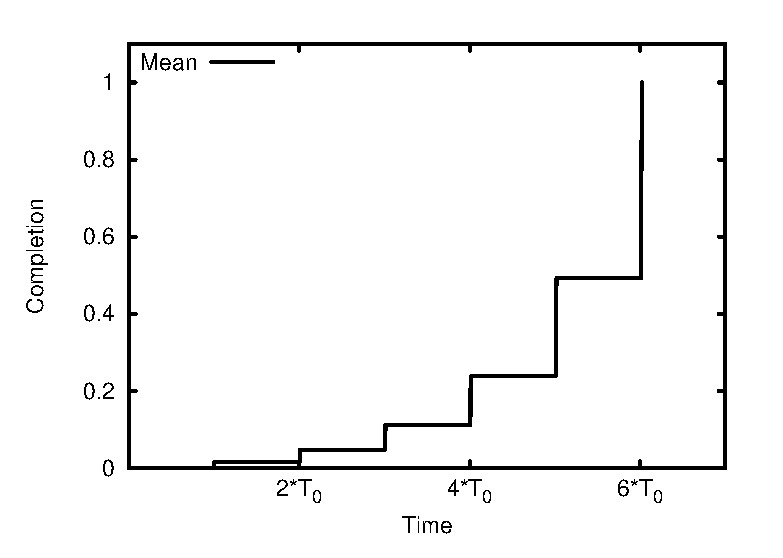
\includegraphics[width=1\textwidth]{fig/plots/scenario_3_log/plots/GeneratedMeanChunkCompletion.csv.eps}
  \end{center}
\end{frame}


\begin{frame}
  \frametitle{Anhang - Szenario Logarithmic}
  Super-Peer Upload Bandwidth:
  
  \begin{center}
    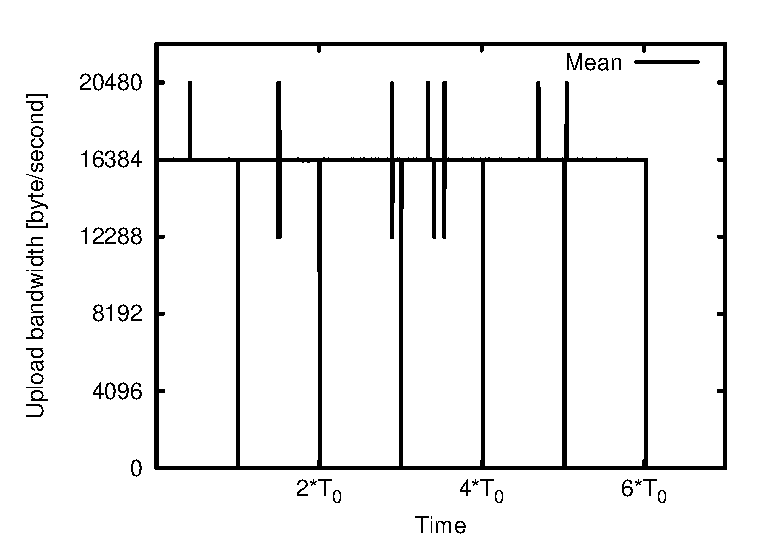
\includegraphics[width=1\textwidth]{fig/plots/scenario_3_log/plots/GeneratedMeanCurrentSuperSeederUploadBandwidth.csv.eps}
  \end{center}
\end{frame}


\begin{frame}
  \frametitle{Anhang - Szenario Logarithmic}
  Peer Upload Bandwidth:
  
  \begin{center}
    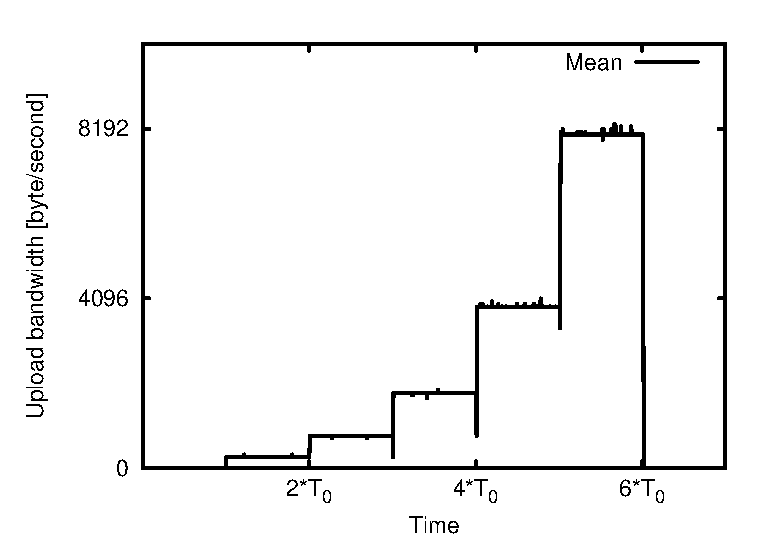
\includegraphics[width=1\textwidth]{fig/plots/scenario_3_log/plots/GeneratedMeanCurrentUploadBandwidth.csv.eps}
  \end{center}
\end{frame}


\begin{frame}
  \frametitle{Anhang - Szenario Logarithmic}
  Peer Download Bandwidth:
  
  \begin{center}
    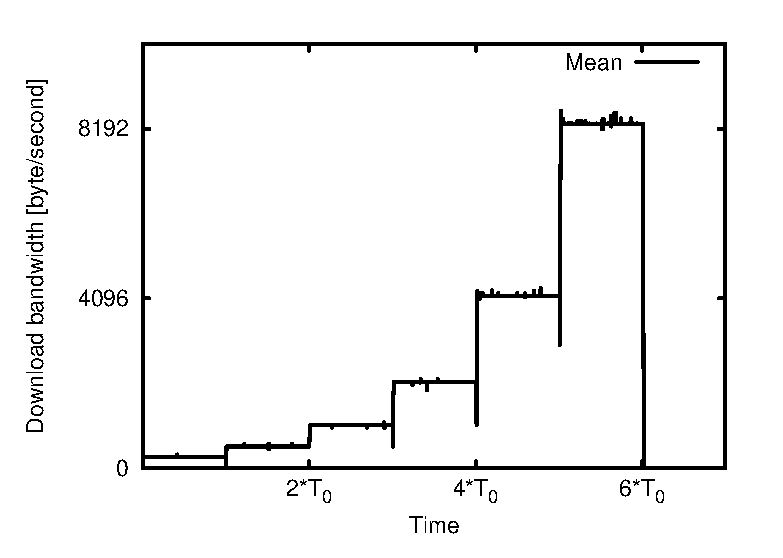
\includegraphics[width=1\textwidth]{fig/plots/scenario_3_log/plots/GeneratedMeanCurrentDownloadBandwidth.csv.eps}
  \end{center}
\end{frame}



%%%
%%% Szenario MetaData 0
%%%

\begin{frame}
  \frametitle{Anhang - Default Szenario mit Meta-Daten 0}
  Completion Graph:
  
  \begin{center}
    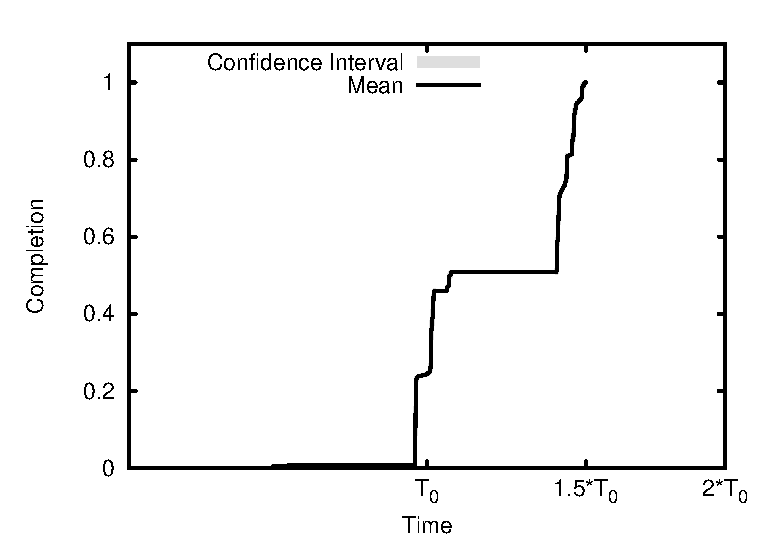
\includegraphics[width=1\textwidth]{fig/plots/scenario_5_meta_data_0/plots/GeneratedMeanChunkCompletion.csv.eps}
  \end{center}
\end{frame}


\begin{frame}
  \frametitle{Anhang - Default Szenario mit Meta-Daten 0}
  Super-Peer Upload Bandwidth:
  
  \begin{center}
    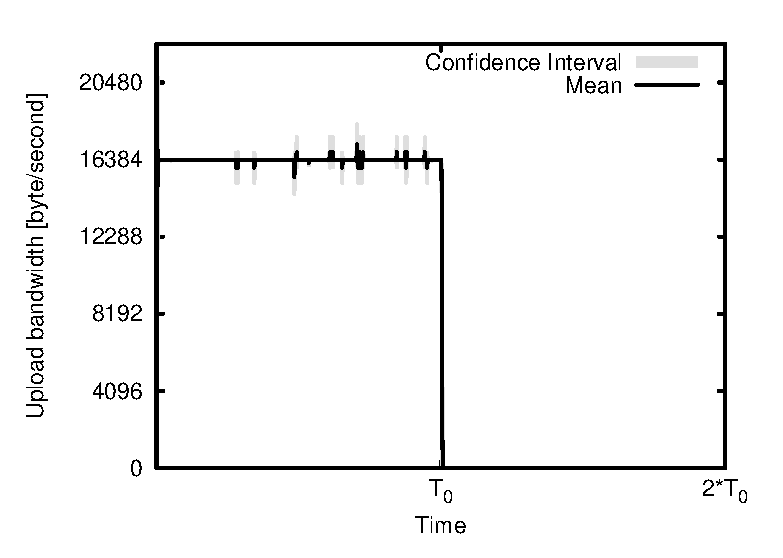
\includegraphics[width=1\textwidth]{fig/plots/scenario_5_meta_data_0/plots/GeneratedMeanCurrentSuperSeederUploadBandwidth.csv.eps}
  \end{center}
\end{frame}


\begin{frame}
  \frametitle{Anhang - Default Szenario mit Meta-Daten 0}
  Peer Upload Bandwidth:
  
  \begin{center}
    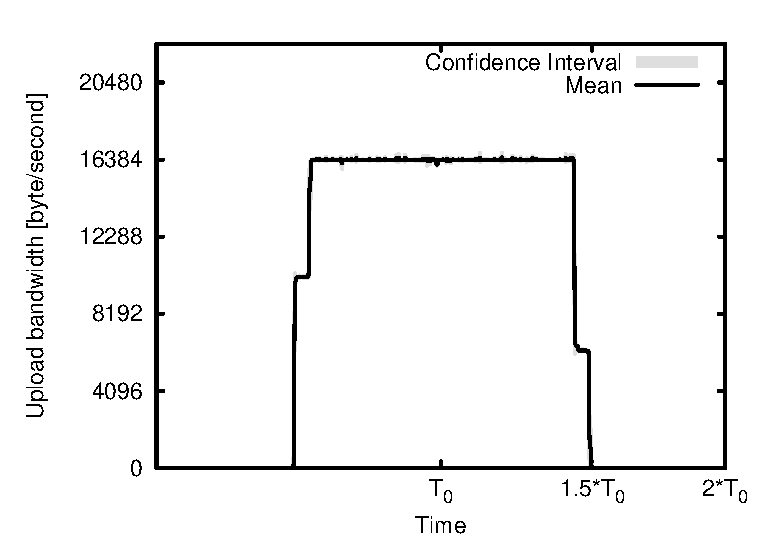
\includegraphics[width=1\textwidth]{fig/plots/scenario_5_meta_data_0/plots/GeneratedMeanCurrentUploadBandwidth.csv.eps}
  \end{center}
\end{frame}


\begin{frame}
  \frametitle{Anhang - Default Szenario mit Meta-Daten 0}
  Peer Download Bandwidth:
  
  \begin{center}
    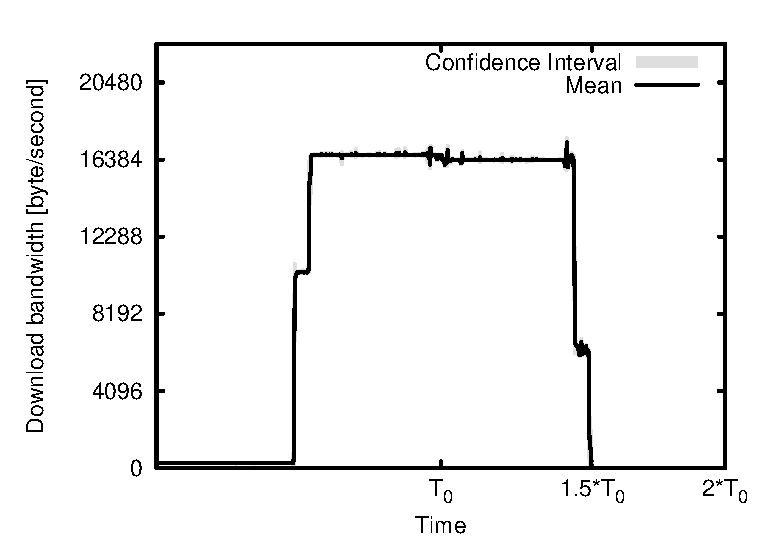
\includegraphics[width=1\textwidth]{fig/plots/scenario_5_meta_data_0/plots/GeneratedMeanCurrentDownloadBandwidth.csv.eps}
  \end{center}
\end{frame}


%%%
%%% Szenario MetaData 10
%%%

\begin{frame}
  \frametitle{Anhang - Default Szenario mit Meta-Daten 10}
  Completion Graph:
  
  \begin{center}
    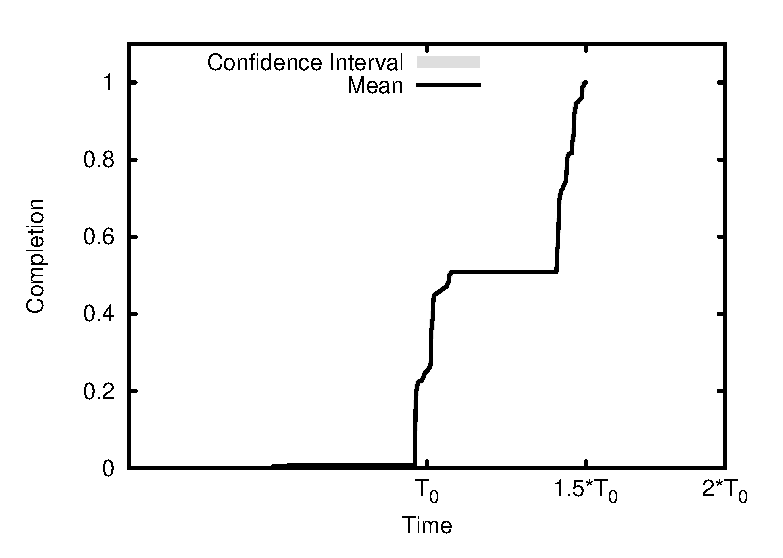
\includegraphics[width=1\textwidth]{fig/plots/scenario_10_meta_data_10/plots/GeneratedMeanChunkCompletion.csv.eps}
  \end{center}
\end{frame}


\begin{frame}
  \frametitle{Anhang - Default Szenario mit Meta-Daten 10}
  Super-Peer Upload Bandwidth:
  
  \begin{center}
    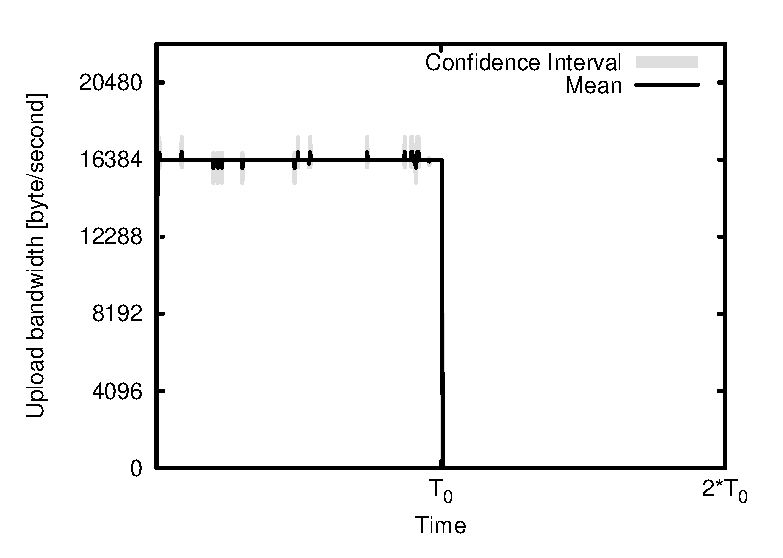
\includegraphics[width=1\textwidth]{fig/plots/scenario_10_meta_data_10/plots/GeneratedMeanCurrentSuperSeederUploadBandwidth.csv.eps}
  \end{center}
\end{frame}


\begin{frame}
  \frametitle{Anhang - Default Szenario mit Meta-Daten 10}
  Peer Upload Bandwidth:
  
  \begin{center}
    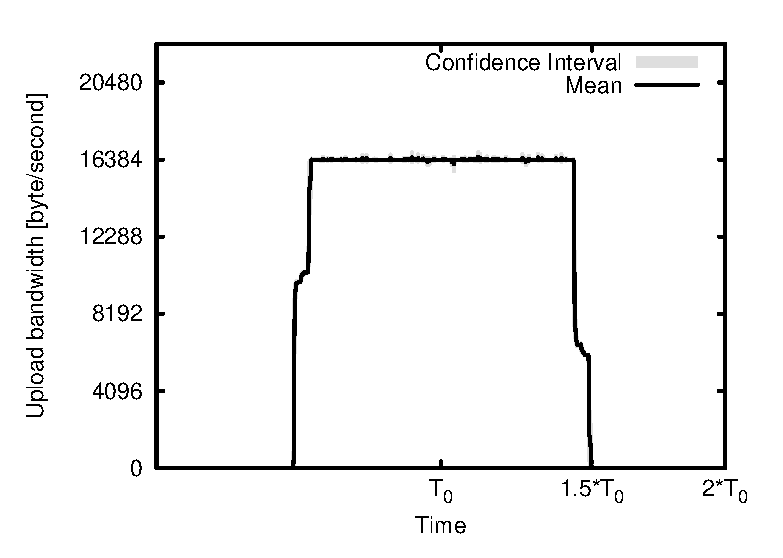
\includegraphics[width=1\textwidth]{fig/plots/scenario_10_meta_data_10/plots/GeneratedMeanCurrentUploadBandwidth.csv.eps}
  \end{center}
\end{frame}


\begin{frame}
  \frametitle{Anhang - Default Szenario mit Meta-Daten 10}
  Peer Download Bandwidth:
  
  \begin{center}
    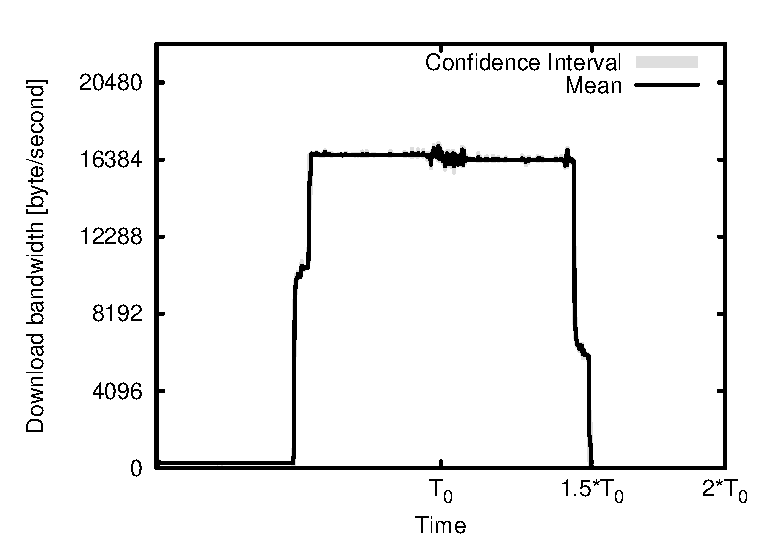
\includegraphics[width=1\textwidth]{fig/plots/scenario_10_meta_data_10/plots/GeneratedMeanCurrentDownloadBandwidth.csv.eps}
  \end{center}
\end{frame}

%%%
%%% Szenario ChunkFac 1
%%%

\begin{frame}
  \frametitle{Anhang - Default Szenario mit 1x Chunkanzahl}
  Completion Graph:
  
  \begin{center}
    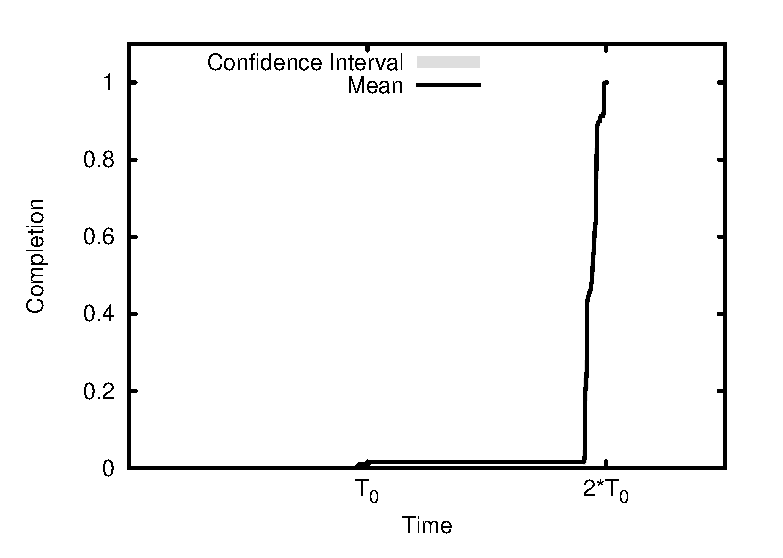
\includegraphics[width=1\textwidth]{fig/plots/scenario_7_chunk_count_fac_1/plots/GeneratedMeanChunkCompletion.csv.eps}
  \end{center}
\end{frame}


\begin{frame}
  \frametitle{Anhang - Default Szenario mit 1x Chunkanzahl}
  Super-Peer Upload Bandwidth:
  
  \begin{center}
    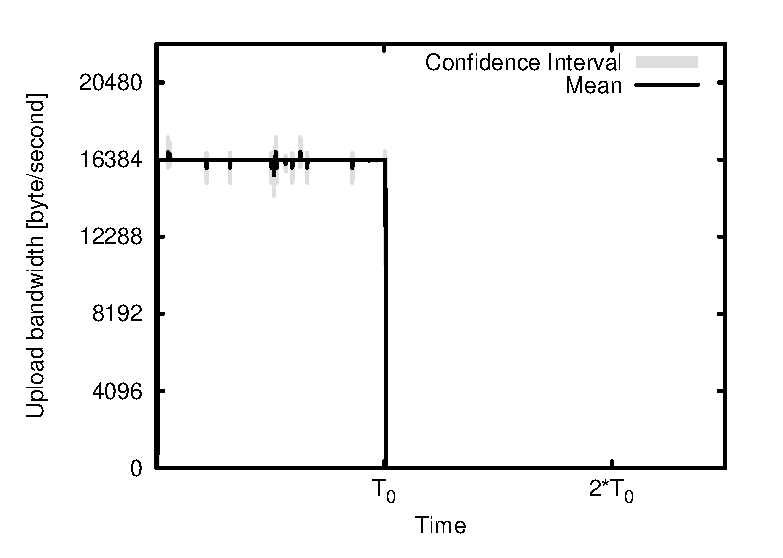
\includegraphics[width=1\textwidth]{fig/plots/scenario_7_chunk_count_fac_1/plots/GeneratedMeanCurrentSuperSeederUploadBandwidth.csv.eps}
  \end{center}
\end{frame}


\begin{frame}
  \frametitle{Anhang - Default Szenario mit 1x Chunkanzahl}
  Peer Upload Bandwidth:
  
  \begin{center}
    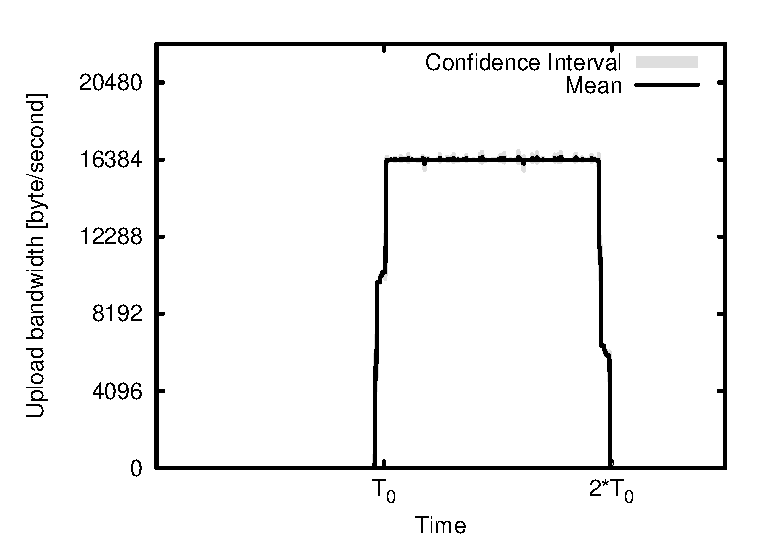
\includegraphics[width=1\textwidth]{fig/plots/scenario_7_chunk_count_fac_1/plots/GeneratedMeanCurrentUploadBandwidth.csv.eps}
  \end{center}
\end{frame}


\begin{frame}
  \frametitle{Anhang - Default Szenario mit 1x Chunkanzahl}
  Peer Download Bandwidth:
  
  \begin{center}
    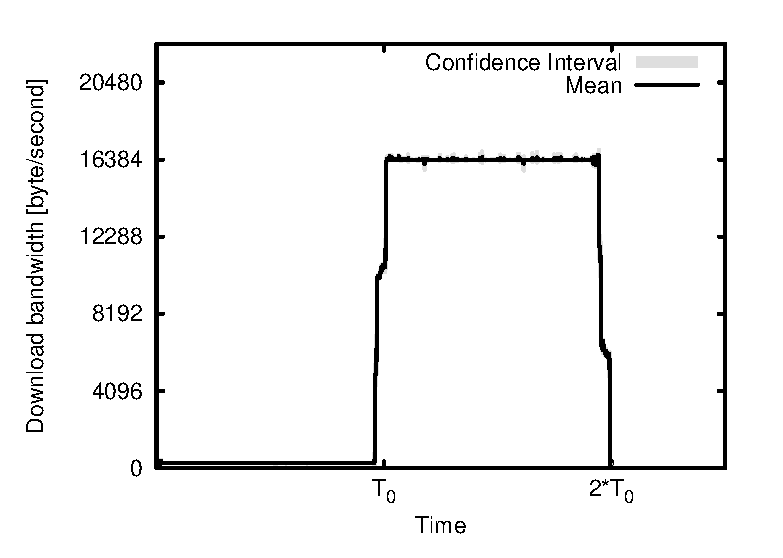
\includegraphics[width=1\textwidth]{fig/plots/scenario_7_chunk_count_fac_1/plots/GeneratedMeanCurrentDownloadBandwidth.csv.eps}
  \end{center}
\end{frame}

%%%
%%% Szenario ChunkFac 8
%%%

\begin{frame}
  \frametitle{Anhang - Default Szenario mit 8x Chunkanzahl}
  Completion Graph:
  
  \begin{center}
    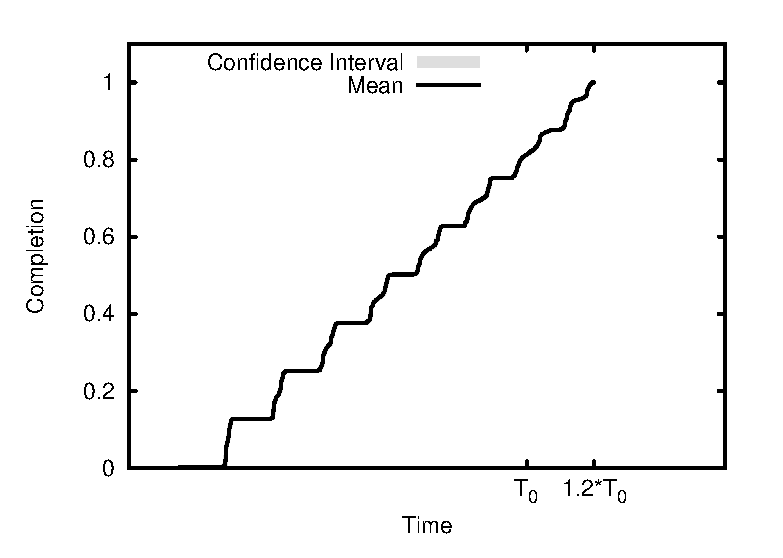
\includegraphics[width=1\textwidth]{fig/plots/scenario_16_chunk_count_fac_8/plots/GeneratedMeanChunkCompletion.csv.eps}
  \end{center}
\end{frame}


\begin{frame}
  \frametitle{Anhang - Default Szenario mit 8x Chunkanzahl}
  Super-Peer Upload Bandwidth:
  
  \begin{center}
    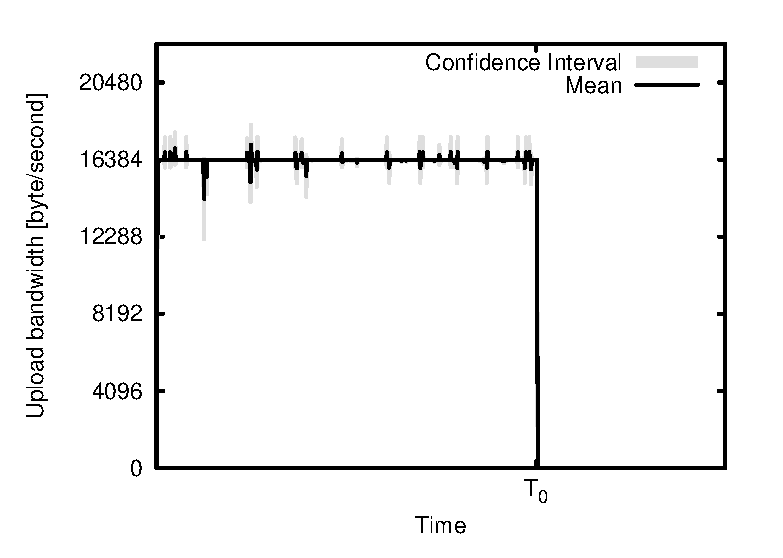
\includegraphics[width=1\textwidth]{fig/plots/scenario_16_chunk_count_fac_8/plots/GeneratedMeanCurrentSuperSeederUploadBandwidth.csv.eps}
  \end{center}
\end{frame}


\begin{frame}
  \frametitle{Anhang - Default Szenario mit 8x Chunkanzahl}
  Peer Upload Bandwidth:
  
  \begin{center}
    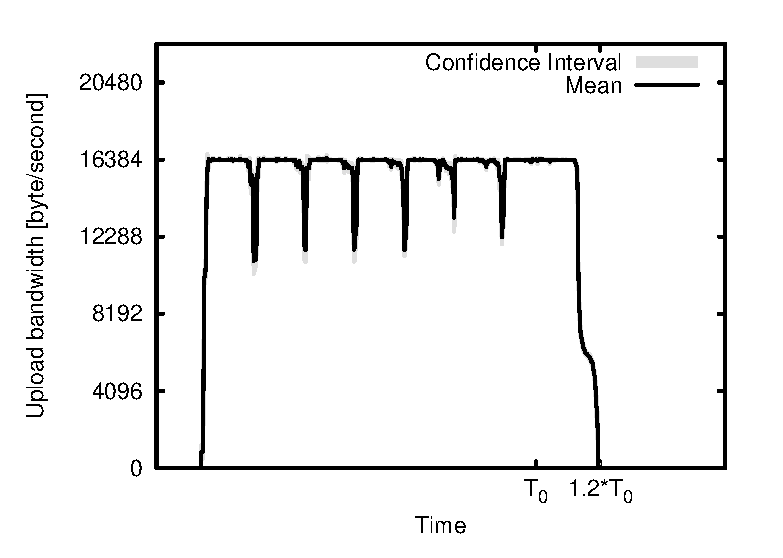
\includegraphics[width=1\textwidth]{fig/plots/scenario_16_chunk_count_fac_8/plots/GeneratedMeanCurrentUploadBandwidth.csv.eps}
  \end{center}
\end{frame}


\begin{frame}
  \frametitle{Anhang - Default Szenario mit 8x Chunkanzahl}
  Peer Download Bandwidth:
  
  \begin{center}
    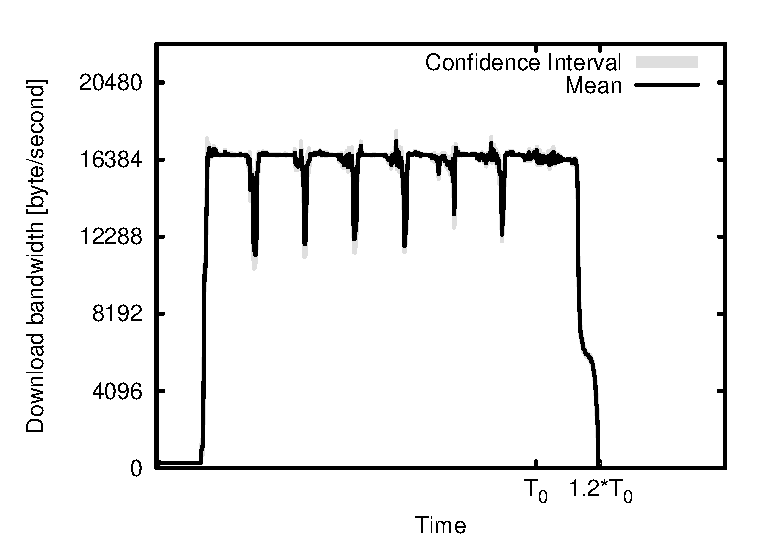
\includegraphics[width=1\textwidth]{fig/plots/scenario_16_chunk_count_fac_8/plots/GeneratedMeanCurrentDownloadBandwidth.csv.eps}
  \end{center}
\end{frame}


%%%
%%% Szenario ChunkFac 16
%%%

\begin{frame}
  \frametitle{Anhang - Default Szenario mit 16x Chunkanzahl}
  Completion Graph:
  
  \begin{center}
    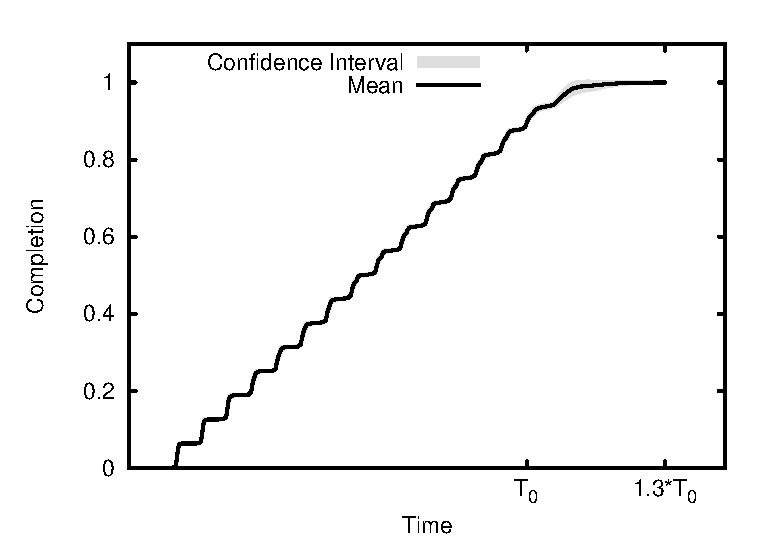
\includegraphics[width=1\textwidth]{fig/plots/scenario_17_chunk_count_fac_16/plots/GeneratedMeanChunkCompletion.csv.eps}
  \end{center}
\end{frame}


\begin{frame}
  \frametitle{Anhang - Default Szenario mit 16x Chunkanzahl}
  Super-Peer Upload Bandwidth:
  
  \begin{center}
    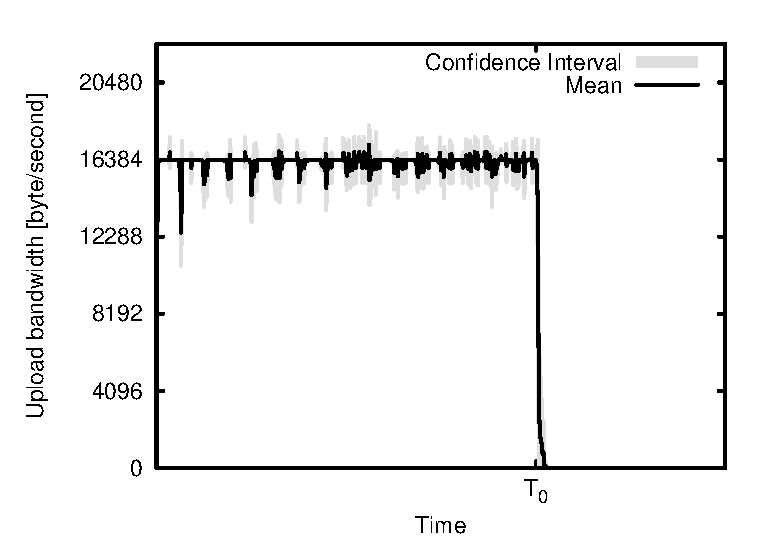
\includegraphics[width=1\textwidth]{fig/plots/scenario_17_chunk_count_fac_16/plots/GeneratedMeanCurrentSuperSeederUploadBandwidth.csv.eps}
  \end{center}
\end{frame}


\begin{frame}
  \frametitle{Anhang - Default Szenario mit 16x Chunkanzahl}
  Peer Upload Bandwidth:
  
  \begin{center}
    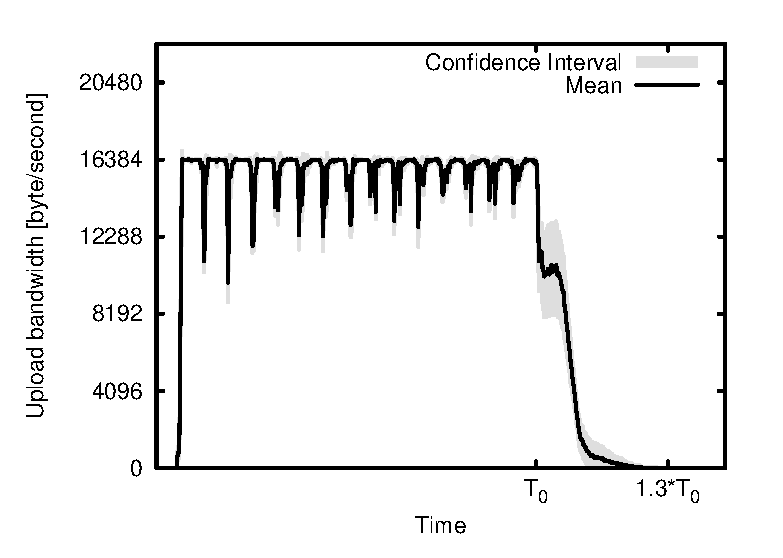
\includegraphics[width=1\textwidth]{fig/plots/scenario_17_chunk_count_fac_16/plots/GeneratedMeanCurrentUploadBandwidth.csv.eps}
  \end{center}
\end{frame}


\begin{frame}
  \frametitle{Anhang - Default Szenario mit 16x Chunkanzahl}
  Peer Download Bandwidth:
  
  \begin{center}
    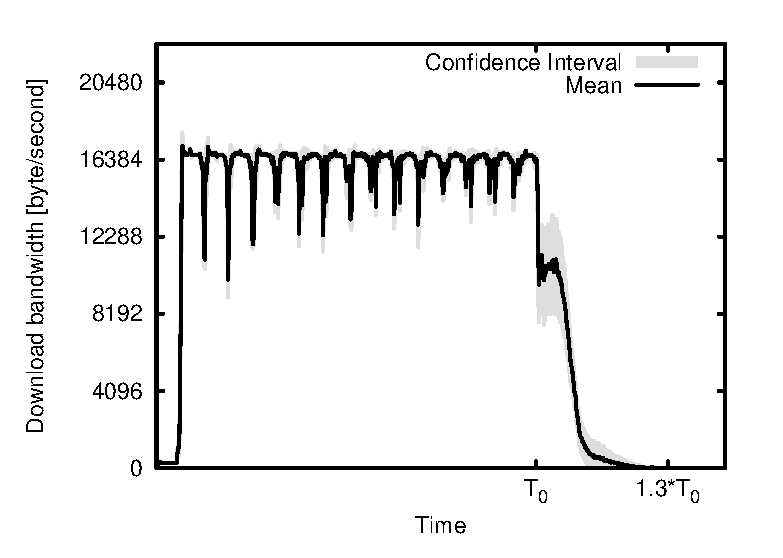
\includegraphics[width=1\textwidth]{fig/plots/scenario_17_chunk_count_fac_16/plots/GeneratedMeanCurrentDownloadBandwidth.csv.eps}
  \end{center}
\end{frame}
